\documentclass{article}

\usepackage{fancyhdr}
\usepackage{extramarks}
\usepackage{amsmath}
\usepackage{amssymb}
\usepackage{enumerate}
\usepackage{graphicx}
\usepackage{pgfplotstable}


% Useful things
\newcommand{\vcenteredinclude}[1]{\begingroup
\setbox0=\hbox{\includegraphics{#1}}%
\parbox{\wd0}{\box0}\endgroup}

%% better: (general command to vertically center horizontal material)
\newcommand*{\vcenteredhbox}[1]{\begingroup
\setbox0=\hbox{#1}\parbox{\wd0}{\box0}\endgroup}

%
% Basic Document Settings
%

\topmargin=-0.45in
\evensidemargin=0in
\oddsidemargin=0in
\textwidth=6.5in
\textheight=9.0in
\headsep=0.25in

\linespread{1.1}

\pagestyle{fancy}
\lhead{\hmwkAuthorName}
\chead{\hmwkClass\ : \hmwkTitle}
\rhead{\firstxmark}
\lfoot{\lastxmark}
\cfoot{\thepage}

\renewcommand\headrulewidth{0.4pt}
\renewcommand\footrulewidth{0.4pt}

\setlength\parindent{0pt}

%
% Create Problem Sections
%

\newcommand{\enterProblemHeader}[1]{
    \nobreak\extramarks{}{Problem \arabic{#1} continued on next page\ldots}\nobreak{}
    \nobreak\extramarks{Problem \arabic{#1} (continued)}{Problem \arabic{#1} continued on next page\ldots}\nobreak{}
}

\newcommand{\exitProblemHeader}[1]{
    \nobreak\extramarks{Problem \arabic{#1} (continued)}{Problem \arabic{#1} continued on next page\ldots}\nobreak{}
    \stepcounter{#1}
    \nobreak\extramarks{Problem \arabic{#1}}{}\nobreak{}
}

\setcounter{secnumdepth}{0}
\newcounter{partCounter}
\newcounter{homeworkProblemCounter}
\setcounter{homeworkProblemCounter}{1}
\nobreak\extramarks{Problem \arabic{homeworkProblemCounter}}{}\nobreak{}

%
% Homework Problem Environment
%
% This environment takes an optional argument. When given, it will adjust the
% problem counter. This is useful for when the problems given for your
% assignment aren't sequential. See the last 3 problems of this template for an
% example.
%
\newenvironment{homeworkProblem}[1][-1]{
    \ifnum#1>0
        \setcounter{homeworkProblemCounter}{#1}
    \fi
    \section{Problem \arabic{homeworkProblemCounter}}
    \setcounter{partCounter}{1}
    \enterProblemHeader{homeworkProblemCounter}
}{
    \exitProblemHeader{homeworkProblemCounter}
}

%
% Homework Details
%   - Title
%   - Due date
%   - Class
%   - Section/Time
%   - Instructor
%   - Author
%

\newcommand{\hmwkTitle}{Homework\ \#6}
\newcommand{\hmwkDueDate}{March 6, 2015}
\newcommand{\hmwkClass}{PHYS 5243 - Solid State Physics}
\newcommand{\hmwkClassInstructor}{Professor Sheena Murphy}
\newcommand{\hmwkAuthorName}{Chase Brown}


\begin{document}
	\begin{homeworkProblem}
		\textbf{Simon - Solid State Basics - Problem 12.1: Crystal Structure of NaCl}
		\hfill
		\\
		Using the Figure 12.21 from Simon's Solid State Basics given below, and given the lattice constant is $a=0.563 nm$, find the following:
		\\
		\centerline{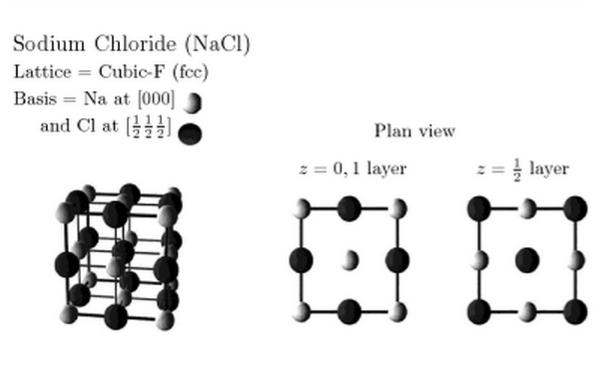
\includegraphics[scale=0.7]{NaCl_Fig.png}}
		\\
		\begin{enumerate}[(a)]
			\item What is the distance from a sodium atom to the nearst chlorine? 
			\item What is the distance from a sodium atom to the nearest other sodium atom?
		\end{enumerate}

		\textbf{Solution}
			\begin{enumerate}[(a)]
				\item The distance from a sodium to the nearest chlorine is along the lattice cell from $[000]$ to $[\frac{1}{2} 00]$ such that the distance between the two atoms is:
					\begin{equation*}
						\boxed{d_{Na\rightarrow Cl} = \frac{1}{2}a = 0.2815nm}
					\end{equation*}
				\item The distance between two nearest neighbor sodium atoms is from $[000]$ to $[\frac{1}{2}\frac{1}{2}0]$ such that the distance between the two atoms is due to the pythagorean theorem:
					\begin{equation*}
						\begin{aligned}
							d_{Na\rightarrow Na} = \sqrt{(\frac{1}{2}a)^2+(\frac{1}{2}a)^2} \\
							= \sqrt{2(\frac{1}{2}a)^2} \\
							=\frac{a}{\sqrt{2}}\\
							\Rightarrow \boxed{d_{Na\rightarrow Na}  = 0.39811 nm}
						\end{aligned}
					\end{equation*}
			\end{enumerate}
	\end{homeworkProblem}
	

	\pagebreak

	\begin{homeworkProblem}
		\textbf{Simon - Solid State Basics - Problem 12.2: Neighbors in the Face-Centered Lattice}
		\hfill
		\\
		\begin{enumerate}[(a)]
			\item Show that similar lattice points in an FCC lattice have 12 nearest neighbors, and find the distance each lattice point is between each other in terms of lattice constant $a$.
			\item Now stretch the sides to an orthorhombic FCC lattice with unit cell side lengths of $a$, $b$, and $c$. What are the distances to each nearest neighbor now, and how many new nearest neighbors are there?
		\end{enumerate}


		\textbf{Solution}
			\begin{enumerate}[(a)]
				\item In each plane there are 4 atoms which have a distance $\frac{a}{\sqrt{2}}$ at a diagonal from the lattice point at the center, as shown by the black lattice points in the figure below:
					\\
					\centerline{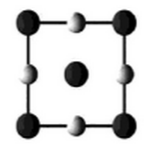
\includegraphics[scale=1]{small_NaCl.png}}
					\\
				We can see that the full 3D structure can have a $[100]$ plane, a $[010]$ plane and a $[001]$ plane put through the middle lattice point and 4 unique atoms will be in the corners with the same type of structure as given in the image above.  This can be seen by disecting the 3D structure into the 3 different planes here:
					\\
					\centerline{
						\vcenteredhbox{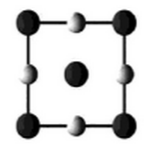
\includegraphics[scale=1]{small_NaCl.png}}
						+ 
						\vcenteredhbox{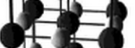
\includegraphics[scale=1]{010plane.png}}
						+
						\vcenteredhbox{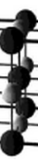
\includegraphics[scale=1]{001plane.png}}
						$\rightarrow$
						\vcenteredhbox{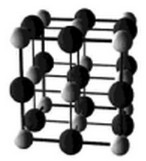
\includegraphics[scale=1]{3D.png}}
					}					
					\\
				Therefore, there are 4 atoms for 3 planes, yeilding 12 unique nearest nieghbor atoms.

				\item Now if we stretch each axis to lengths $a$, $b$, and $c$, we can see that the same pythagorean law applies, but now each side has a different length in each plane and we end up with the following values for each distance in each plane:
				\begin{equation*}
					\begin{aligned}
						d_{[100]} = \frac{\sqrt{a^2+b^2}}{2} \\
						d_{[010]} = \frac{\sqrt{a^2+c^2}}{2} \\
						d_{[001]} = \frac{\sqrt{b^2+c^2}}{2}
					\end{aligned}
				\end{equation*}
					Now that there are 3 different lengths for each plane, we can see that only one of these lengths will be the smallest, and therefore only the 4 atoms in that plane will be the nearest neighbors for that lattice point.

			\end{enumerate}

		
	\end{homeworkProblem}

	\pagebreak

	\begin{homeworkProblem}
		\textbf{Simon - Solid State Basics - Problem 12.3: Crystal Structure}
		\hfill
		\\
		Figure 12.22 from Simon's Solid State Basic's is given below for Zinc Blende (ZnS). The numbers are heights of the atoms above the $z=0$ axis as fractions of lattice constant $a$. Unlabeled atoms are at $z=0$ and $z=a$.
		\\
			\centerline{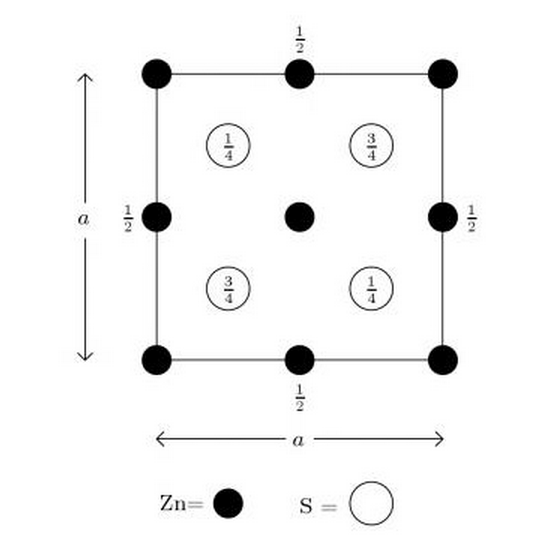
\includegraphics[scale=0.6]{ZnS.png}}
		\\
		\begin{enumerate}[(a)]
			\item What is the Bravais lattice type?
			\item Describe the basis.
			\item Given that $a=0.514 nm$, calculate the nearest-neighbor Zn-Zn, Zn-S, and S-S distances.
		\end{enumerate}
		

		\textbf{Solution}
			\begin{enumerate}[(a)]
				\item The Bravais Lattice is Face-Centered Cubic
				\item The basis is based on two atoms - 1 Zn atom and 1 S atom - situated at the origin for Zn [000], and $[\frac{1}{4}\frac{-1}{4} \frac{1}{4}]$ for the Sulfur atom.
				\item The nearest-neighbor distances can be calculated using the pythagorean theorem much in the same way it was done for problems 12.1 and 12.2:
						\begin{equation*}
							\begin{aligned}
								\boxed{d_{Zn-Zn} = \frac{a}{\sqrt{2}}} \\
								\boxed{d_{Zn-S} = \frac{\sqrt{3}a}{4}} \\
								\boxed{d_{S-S} = \frac{a}{\sqrt{2}}}
							\end{aligned}
						\end{equation*}
			\end{enumerate}

	\end{homeworkProblem}

	\pagebreak

	\begin{homeworkProblem}
		\textbf{Simon - Solid State Basics - Problem 12.4: Packing Fractions}
		\hfill
		\\
		Consider a lattice with a sphere at each lattice point. Choose a radius such that the neighboring spheres touch. The  packing fraction is the ratio of the volume occupied by the spheres to the total volume of the cube. Find the packing fractions for the following structures:
		\begin{enumerate}[(a)]
			\item Simple Cubic Lattice.
			\item Body Centered Cubic Lattice.
			\item Face Centered Cubic Lattice.
		\end{enumerate}
		

		\textbf{Solution}\\
			The standard equation for the atomic packing factor is:
			\begin{equation*}
				\eta = \frac{N (\frac{4}{3}\pi r(a)^3)}{a^3}
			\end{equation*}
			Where $\eta$ is the atomic packing factor, $N$ is the number of atoms within the unit cell, $a$ is the lattice constant, and $r(a)$ is the radius of the atom in terms of $a$. 
			\begin{enumerate}[(a)]
				\item The simple cubic lattice will have tthe following atomic packing factor as $N=1$, and $r(a) = \frac{a}{2}$ as seen from the unit cell below:
				\begin{equation*}
					\boxed{\eta_{SC} = \frac{\pi}{6} \approx 0.52}
				\end{equation*}
				\\
					\centerline{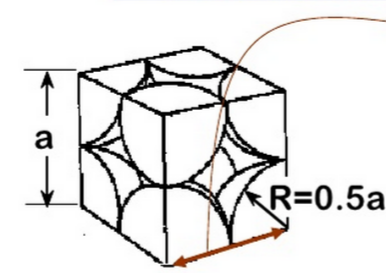
\includegraphics[scale=1]{SC.png}}
				\\
				
				\item The BCC lattice has $N=2$, and $r(a)=\frac{\sqrt{3}a}{4}$ as can be seen by fnding the diagonal length through the unit cell.
				\begin{equation*}
					\boxed{\eta_{BCC} = \frac{3^{\frac{3}{2}}\pi}{24} \approx 0.68}
				\end{equation*}
				\\
					\centerline{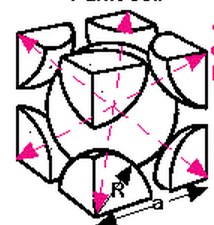
\includegraphics[scale=1]{BCC.png}}
				\\
				

				\item The FCC lattice has $N=4$, and $r(a)=\frac{\sqrt{2}a}{4}$ as can be seen by fnding the diagonal length through the unit cell.
				\begin{equation*}
					\boxed{\eta_{FCC} = \frac{2^{\frac{3}{2}}\pi}{12} \approx 0.74}
				\end{equation*}
				\\
					\centerline{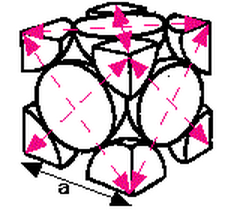
\includegraphics[scale=1]{FCC.png}}
				\\

			\end{enumerate}

	\end{homeworkProblem}

\pagebreak

	\begin{homeworkProblem}
		\textbf{Simon - Solid State Basics - Problem 12.5: Fluorine Beta Phase}
		\hfill
		\\
		Fluorine can crystallize into a betaphase at $45-55K$. Below is the structure for this beta phase:
		\\
			\centerline{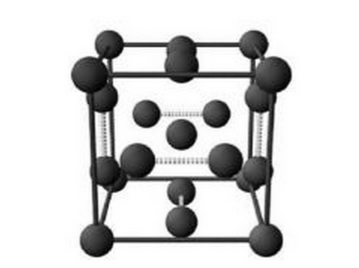
\includegraphics[scale=1]{Fluorine.png}}
		\\

		\begin{enumerate}[(a)]
			\item How many atoms are in this conventional unit cell?
			\item What is the lattice and the basis for this crystal?
		\end{enumerate}
		
		\textbf{Solution}
			\begin{enumerate}[(a)]
				\item The number of atoms within the unit cell is 8.  This can be seen from the 2 half atoms coupled along the sides giving 6 atoms, the one in the center, and the corners giving another atom.
				\item This lattice is Simple Cubic.
			\end{enumerate}
	\end{homeworkProblem}

\pagebreak

	\begin{homeworkProblem}
		\textbf{Simon - Solid State Basics - Problem 13.3: Directions and Spacings of Crystal Planes}
		\hfill
		\begin{enumerate}[(a)]
			\item Explain what is meant by 'crystal planes' and 'Miller Indices'.
			\item Show that the general direction $[hkl]$ in a cubic crystal is normal to the planes with Miller Indices $(hkl)$.
			\item Is the same true in general for an orthorhombic crystal?
			\item Show that the spacing $d$ of the $(hkl)$ set of planes in a cubic crystal with lattice parameter
$a$ is
			\begin{equation*}
				d = \frac{a}{\sqrt{h^2+k^2+l^2}}
			\end{equation*}
			\item What is the generalization of this formula for an orthorhombic crystal?
		\end{enumerate}
		
		\textbf{Solution}
			\begin{enumerate}[(a)]
				\item A crystal plan is a 2 dimensional plane which links lattice points within a crystal lattice structure. Miller indices are the notiation used to describe crystal planes by describing the inverse intersection points with which the plane will intersect the basis vectors describing the lattice.
				\item The Miller Indices are chosen to be the perpendicular to the crystal plane by taking the inverse of where the intersection of the plane is with each basis vector.  We can look at vectors for the three points we have where the plane intersects the axes, $P_1(\frac{1}{h},0,0)$, $P_2(0,\frac{1}{k},0)$ and $P_3(0,0,\frac{1}{l})$.  Now we have two vectors which will define the plane:
		$$ a = \left(\begin{matrix} x_2-x_1\\y_2-y_1\\z_2-z_1 \end{matrix} \right) \qquad b = \left(\begin{matrix} x_3-x_1\\y_3-y_1\\z_3-z_1 \end{matrix} \right) $$ therefore $a = -\frac{1}{h}i+\frac{1}{k}k$, and $b=-\frac{1}{h}i+\frac{1}{l}j$ $$ a\times b = \left|\begin{matrix} i & j & k \\ -\frac{1}{h} & 0 & \frac{1}{k} \\ -\frac{1}{h} & 0 & \frac{1}{l} \\ \end{matrix}\right| =   \left(\begin{matrix} \frac{1}{kl}\\\frac{1}{hl}\\\frac{1}{hl} \end{matrix} \right)$$
			\end{enumerate}
	\end{homeworkProblem}

\pagebreak

	\begin{homeworkProblem}
		\textbf{X-ray Powder Diffraction}
		\hfill
		\\
		X-ray powder diffractions are done for 3 crystals. Each crystal is formed by one kind of atom. The atoms in the three crystals form a simple subic, FCC, and BCC structure. Let $\phi$ be the diffraction angle. The observed diffraction peaks at the following angles for the 3 crystals is given in the tabulated data below.
		\begin{enumerate}[(a)]
			\item Identify the crystal structure of the crystals A, B, and C.
			\item Sketch the first four diffraction peaks for the simple cubic crystal.  Now assume that as we lower the temperature the SC crystal is changed into a tetragonal structure through a continuous phase transition. Describe and sketch how the above four peaks change as the crystal changes into the tetragonal structure.
		\end{enumerate}
		
		\textbf{Solution}\\
			The tabluated data yeilds the following information:

			\begin{enumerate}[(a)]
				\item 
			\end{enumerate}
	\end{homeworkProblem}

\end{document}
